\documentclass{gescons}

\genre {Entrevista}
\author{Keiko Asaoka, Marcos Akira Hattori, Marta Yoshie Takahashi, Michelle Hirata Lopes, Oscar Kenji Nihei e Renata Aoki}
\authorrole{Organizadores}
\title{The English-Japanese Mini-Glossary of Conscientiology Terms}

\begin{document}
    \makeentrevistatitle
    \coverart{back/Mini-Glossary.png}

    \begin{multicols}{2}

\begin{center}
    \vspace{-0.5cm}
    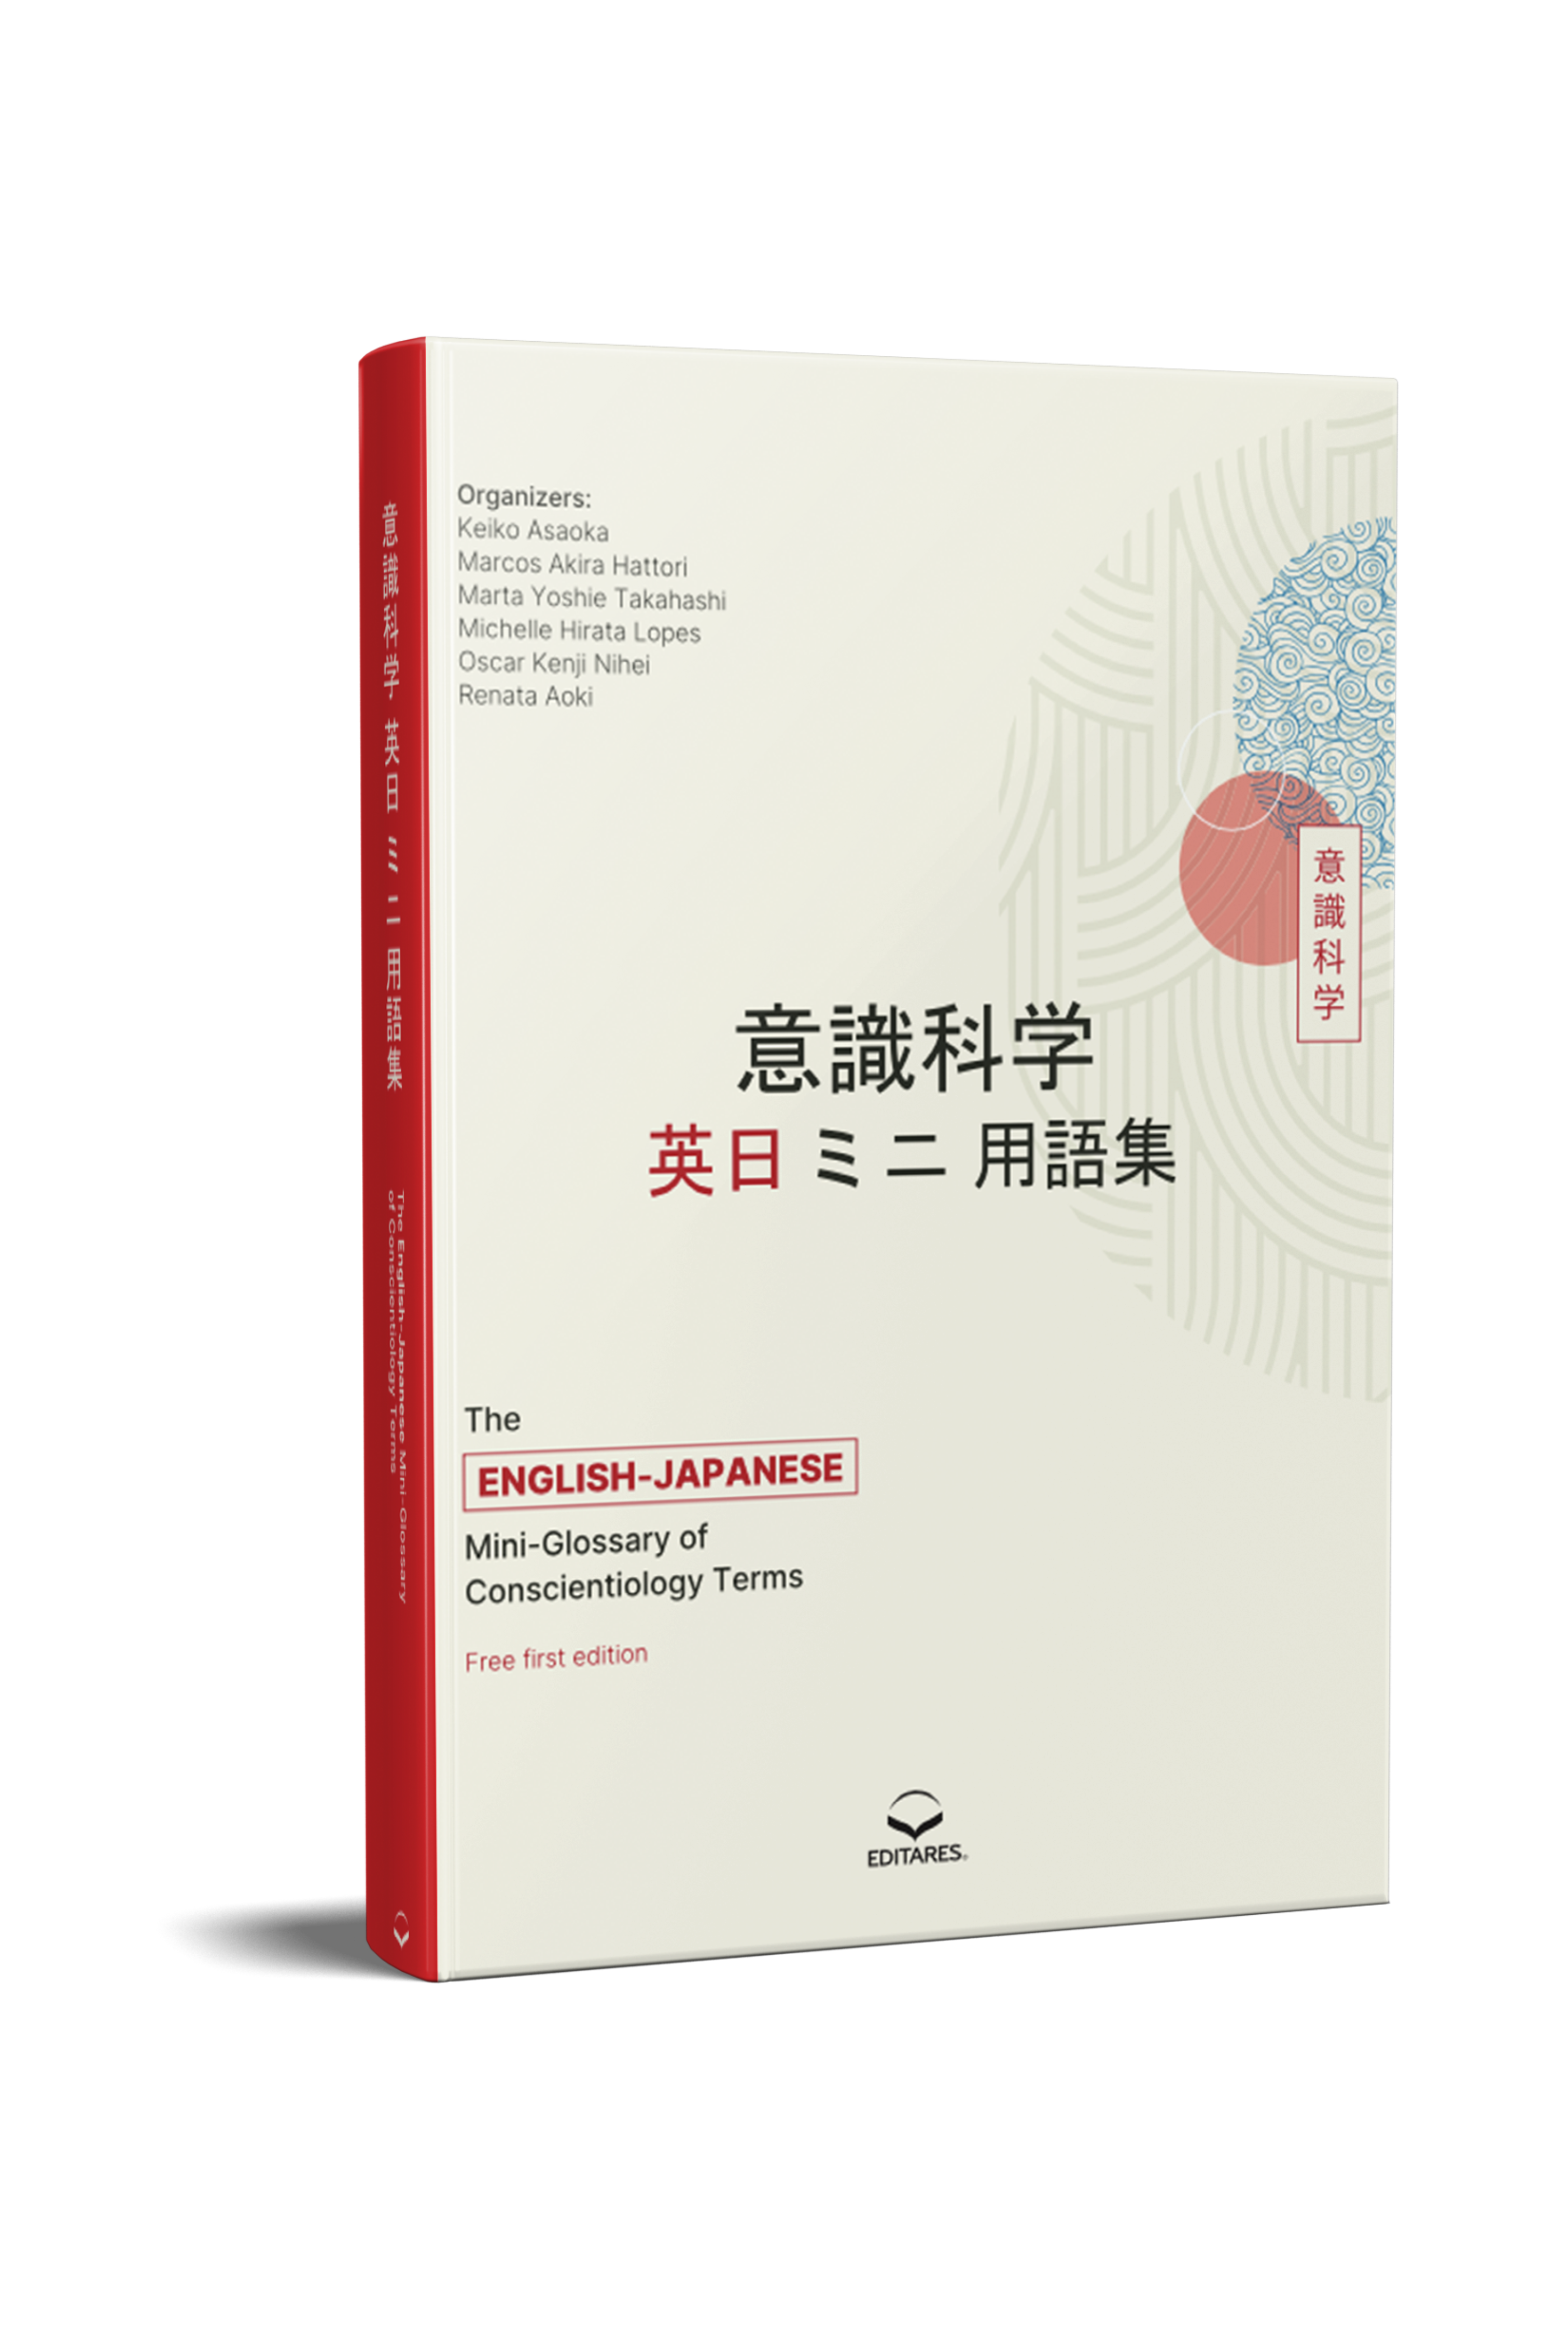
\includegraphics[width=6cm]{articles/entrevista/mockups/Mini-Glossary.png}
\end{center}


\textbf{1. Qual foi a motivação para a escrita da obra? Por que a definição deste tema para publicação de um livro?}

O grupo de voluntários da Nipoteca da Holoteca iniciou os trabalhos de tradução dos termos conscienciológicos para o idioma japonês, a partir de fevereiro de 2024, motivado em permitir o acesso a esses termos e consequentemente à Conscienciologia, aos japoneses e falantes do idioma, tendo como meta a tradução de 600 termos. O que impulsionou como meta a escrita do Miniglossário para a sua publicação, contendo 40 termos essenciais, foi o desafio lançado pela Equipe da Expedição Paracientifica Expo Osaka 2025 - Pró Megacentro Cultural Holoteca, a fim de ser distribuído durante a visita ao Japão, que ocorreu no período de 11 a 24 de maio de 2025.

\begin{pullquote}
    ``O que impulsionou como meta a escrita do Miniglossário para a sua publicação (...) foi o desafio lançado pela Equipe da Expedição Paracientifica Expo Osaka 2025.''
\end{pullquote}

\textbf{2. Quais foram as principais percepções, intra e extrafísicas, durante a pesquisa e a escrita da obra? E posterior ao lançamento?}


Em relação às percepções intrafísicas, desde o início dos trabalhos de tradução, verificou-se que o trabalho com foco interassistencial, foi atrator de novos membros com afinidade com a cultura e idioma japonês para o grupo, que passaram a integrar os trabalhos, que mostraram motivação, comprometimento, responsabilidade e dedicação para a conclusão do miniglossário.

Em relação às percepções extrafísicas, percebeu-se inspirações e sustentação energética dos amparadores extrafísicos, além de sincronicidades ao trabalho, como a realização da viagem ao Japão, chegada de pessoas fundamentais ligadas às Editares, motivados em auxiliar na conclusão do Miniglossário.

\textbf{3. Qual o maior aprendizado com a escrita desta obra?}

Trabalho coeso em equipe, otimização máxima do tempo dedicado à pesquisa e escrita da obra, a importância da estruturação de cronograma objetivo, com metas e prazos definidos. Aprimoramento dos métodos de trabalho em grupo na distribuição das tarefas de tradução e revisão dos termos.


\textbf{4. O que poderiam dizer como incentivo para que mais pesquisadores invistam na publicação de obras conscienciológicas?}

Satisfação íntima e sentimento de completismo grupal, senso de produtividade e do dever cumprido, decorrentes da realização da publicação grupal. Tendo disposição, com metas e cronograma bem definidos, o trabalho se concretiza.

    \end{multicols}
\end{document}
